\documentclass{article}
\usepackage{appendix}
\usepackage{graphicx}
\usepackage{pdfpages}
\usepackage{fullpage}
\usepackage{hyperref}

\title{Architecture Reconstruction: Zeegu-React \\ \normalsize Software Architecture, MSc (Spring 2024) \\ KSSOARC2KU \\}
\author{Bjarke Brodin Larsen -- bjal@itu.dk}


\begin{document}
\maketitle
\tableofcontents

\clearpage
\section{Introduction}

\href{https://zeeguu.com}{Zeegu} is a language learning assistance tool
that helps users learn by reading and revising previously read language on a word-by-word basis.
It contains serveral features such as tracking progress and providing material for language learning
with on demand translations.

\vspace*{1em}\noindent
The front-end of Zeegu is the subject matter of this paper.
More specifically, I attempt to recover information about its architecture,
and subsequently reflect on the results of said recovery.

\section{Methodology: tooling and process step-by-step}

In the following section I will describe which tools I 
deployed in what order and why I chose to do so.

\subsection{Getting acquainted with the system -- ChatGPT}

Because getting hints and ideas about the elephant we are attempting to 
map out is not dependent on precision and in the beginning is mostly a
text-parsing task, I utilized ChatGPT\cite{gpt4} to summarize the
contents of the repository and get an introductory idea 
(see Appendix \ref{apx:a}).
Because ChatGPT can search the web it surprised me by being adept at 
suggesting tools for further inspection which might have come in handy!

\subsection{Getting a more exact feel of function -- running the system}

After quickly getting some hints and a notion about what system I am dealing with,
I proceed to run the system using the online beta deployment hosted at \href{https://zeeguu.com}{https://zeeguu.com}.
This is mostly to probe the system functionality and improve my mental map of how the codebase manifests to the user.

\subsection{Researching and briefly parsing the code manually}

By reviewing and researching the React framework on which the subject codebase is built,
and subsequently simply looking at the code. 
I attempt to acquire a feel for how the code fits together,
how are string translations handled,
how are components themed and global variables managed,
how is routing done.

\subsection{Mining data and producing a module view -- python3, networkx, pyvis}
\label{mining}

With a pretty good idea about the overall system structure,
I begin semi-automatically attempting to map the codebase using python.
Code can be found at \href{https://github.com/bjarkebrodin/recovery}{https://github.com/bjarkebrodin/recovery},
or if for some reason inaccessible is also uploaded as an appendix (see Appendix \ref{apx:b}).
I do this by first extracting the imports between files (see Figure \ref{fig:d:raw})
then subsequently I abstract to top-level modules and consider only imports in between such modules (see Figure \ref{fig:d:abs} and Figure \ref{fig:d:clean}).
This approach is very similar to the one demonstrated by Mircea Lungo in the reconstruction lectures\cite{reconstruction}.
These networks are visualized dynamically as html files and the reader can inspect them at will from the repository,
to make the data inspectable they are programmed with tooltips that show detailed information about nodes (see Figure \ref{fig:d:nodetooltip}), and edges (see Figure \ref{fig:d:edgetooltip}).
I visualize the gathered data and attempt to infer interesting facts about the architecture.
The outcome of this step is described in more detail throughout the remainder of this paper.
I use the tools \verb|pyvis|\cite{pyvis} and \verb|networkx|\cite{networkx} to help me do this without implementing graphs and visualisation myself.

\subsection{Superficially assesing external dependency health -- npm audit}

As a finishing step, only because it is so easily available in npm projects:
to quickly ascertain the health of external dependencies used I run \verb|npm audit|
to get an idea about how much (potential) debt there might be in the way external dependencies are used.



\section{Results}

% outline functionality of zeegu in a bit more detail?


Through semi-automatically eliciting an approximate dependency (JavaScript \verb|import|) structure of the codebase
(as described in Section \ref{mining}),
I produce a module view of the Zeegu front-end (see Figure \ref{fig:3:clean}).

\begin{figure}[h]
  \centering 
  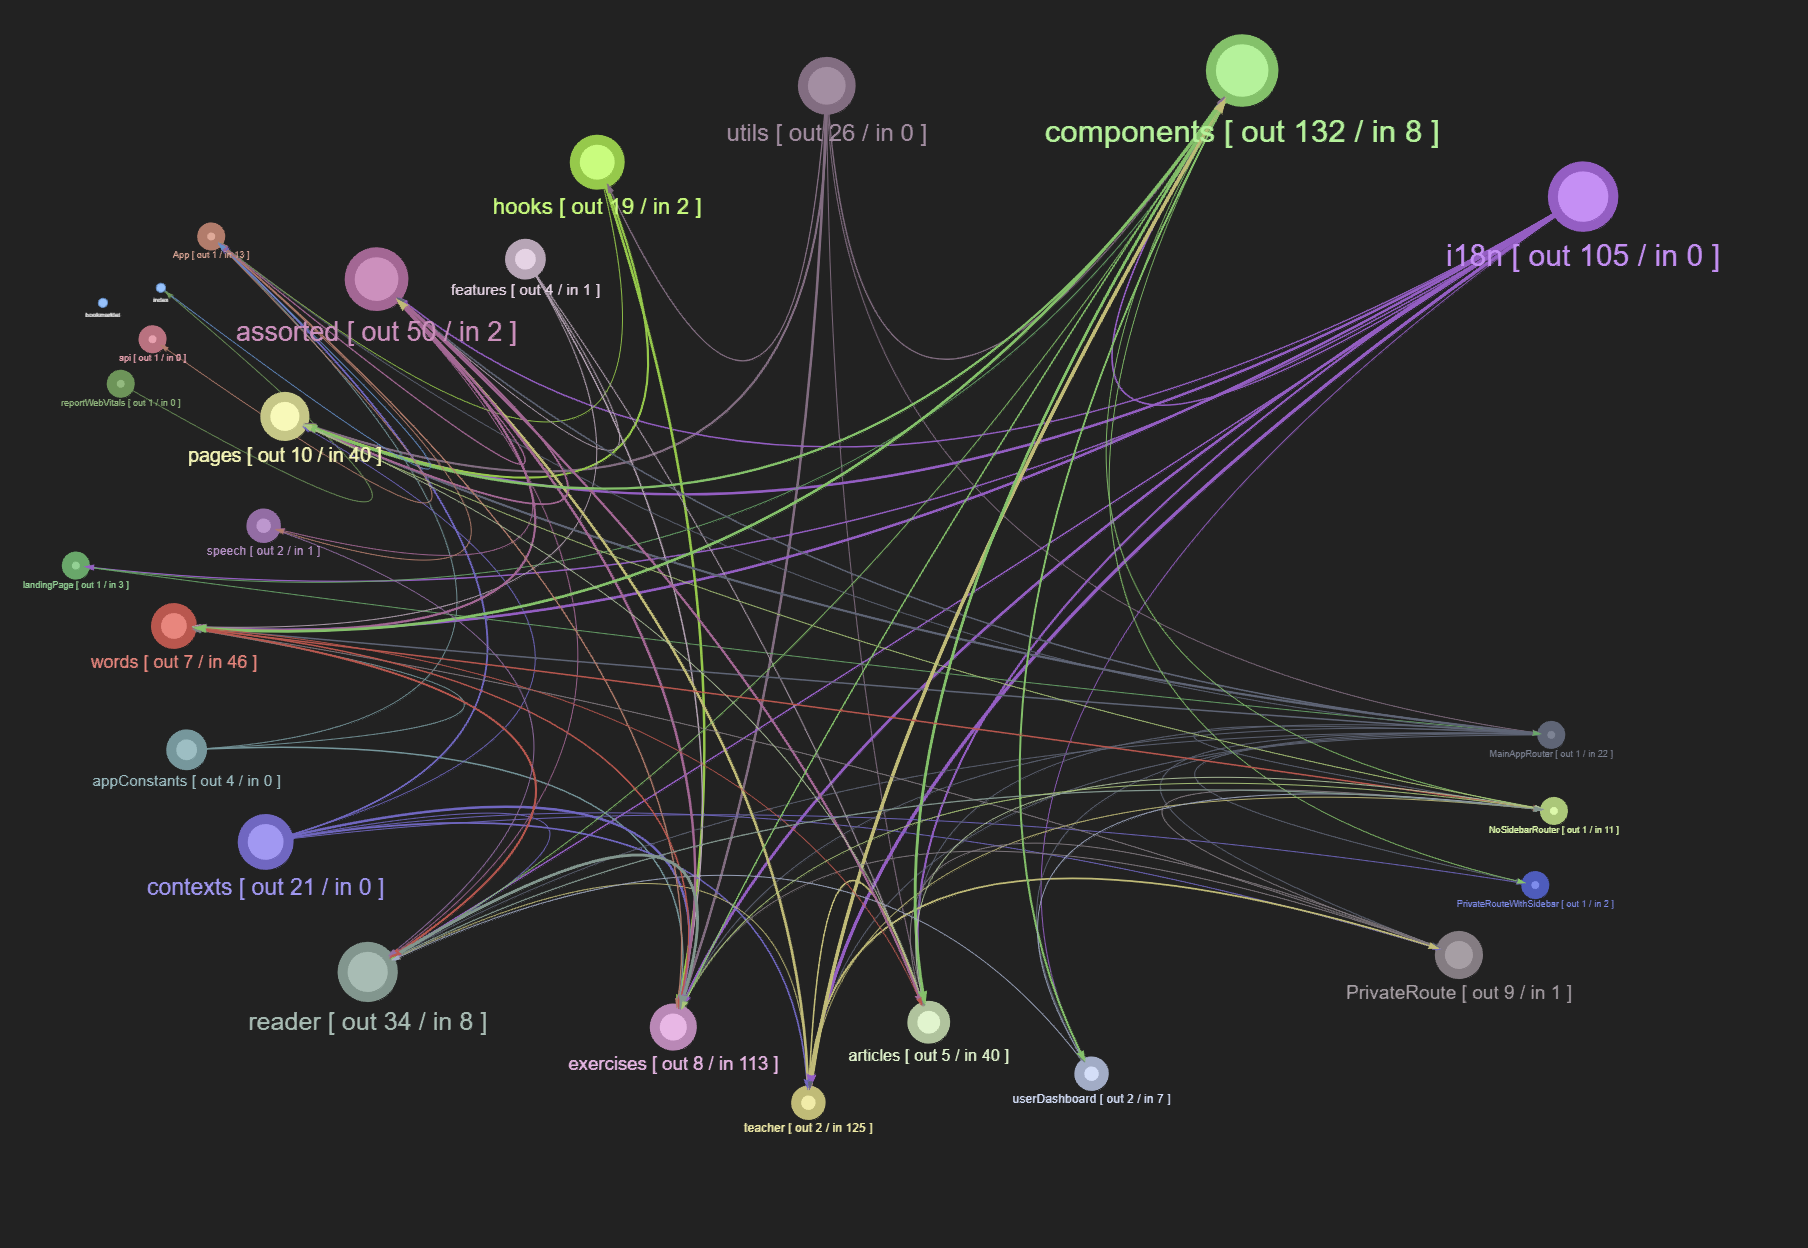
\includegraphics[width=\textwidth]{graphics/module_abstraction_cleaned.png}
  \caption{Cleaned and colored visualisation of all import statements abstracted to top-level modules. 
  Thicker edges represent more imports (logarithmically scaled) and edge 
  direction represents which what is being imported to where.
  Colors do not have meaning but are meant to help better decode the network by eye.
  Modules are appended with information about how many times they are imported and how many times they import another module.
  A bigger circle means a module is imported more times by other modules (\textit{out} value),
  i.e. might be important or central to the architecture. \\ \vspace*{.25em} \\
  \hspace*{2em}\textit{out} -- times imported in a different top-level module \\
  \hspace*{2em}\textit{in} -- times importing a from different top-level module}
  \label{fig:3:clean}
\end{figure}

To frame the information presented in Figure \ref{fig:3:clean} and prime the reader 
for a brief discussion of this data (Section \ref{discussion}),
I briefly cover the purpose of some of the modules.

% i18n
% components
% routers
% hooks, utils, words



\section{Discussion}
\label{discussion}

From visualising and inspecting the data more closely (see Figure \ref{fig:3:clean}), 
both by looking at the overview but also by interacting with 
\href{https://github.com/bjarkebrodin/recovery/blob/master/top_lvl_imports.html}{the generated html}
to inspect exactly what imports what,
I consider a few aspects of the system.

% what would we guess the main role of the front-end architecture is?
% - easily add new routes?
% - easily iterate and develop: modifiability?
% - easily collaborate: open source?
% is component theme coherent across different components?
% is component data-interface separated from component visuals?
% can components be changed without modifying where they appear?
% i18n coupled heavily to codebase?
% seems logically well-grouped but not structurally well decoupled, expand
% - many top-level modules have cross-dependencies, largely not structured as suppliers/consumers
% - better import hierarchy might be nice
% How coupled is routing to pages themselves?
% - could we do this better?


\clearpage
\bibliography{lit}
\bibliographystyle{ieeetran}

\clearpage
\appendix
\section{ChatGPT Transcript}
\label{apx:a}
\begin{figure}[h]
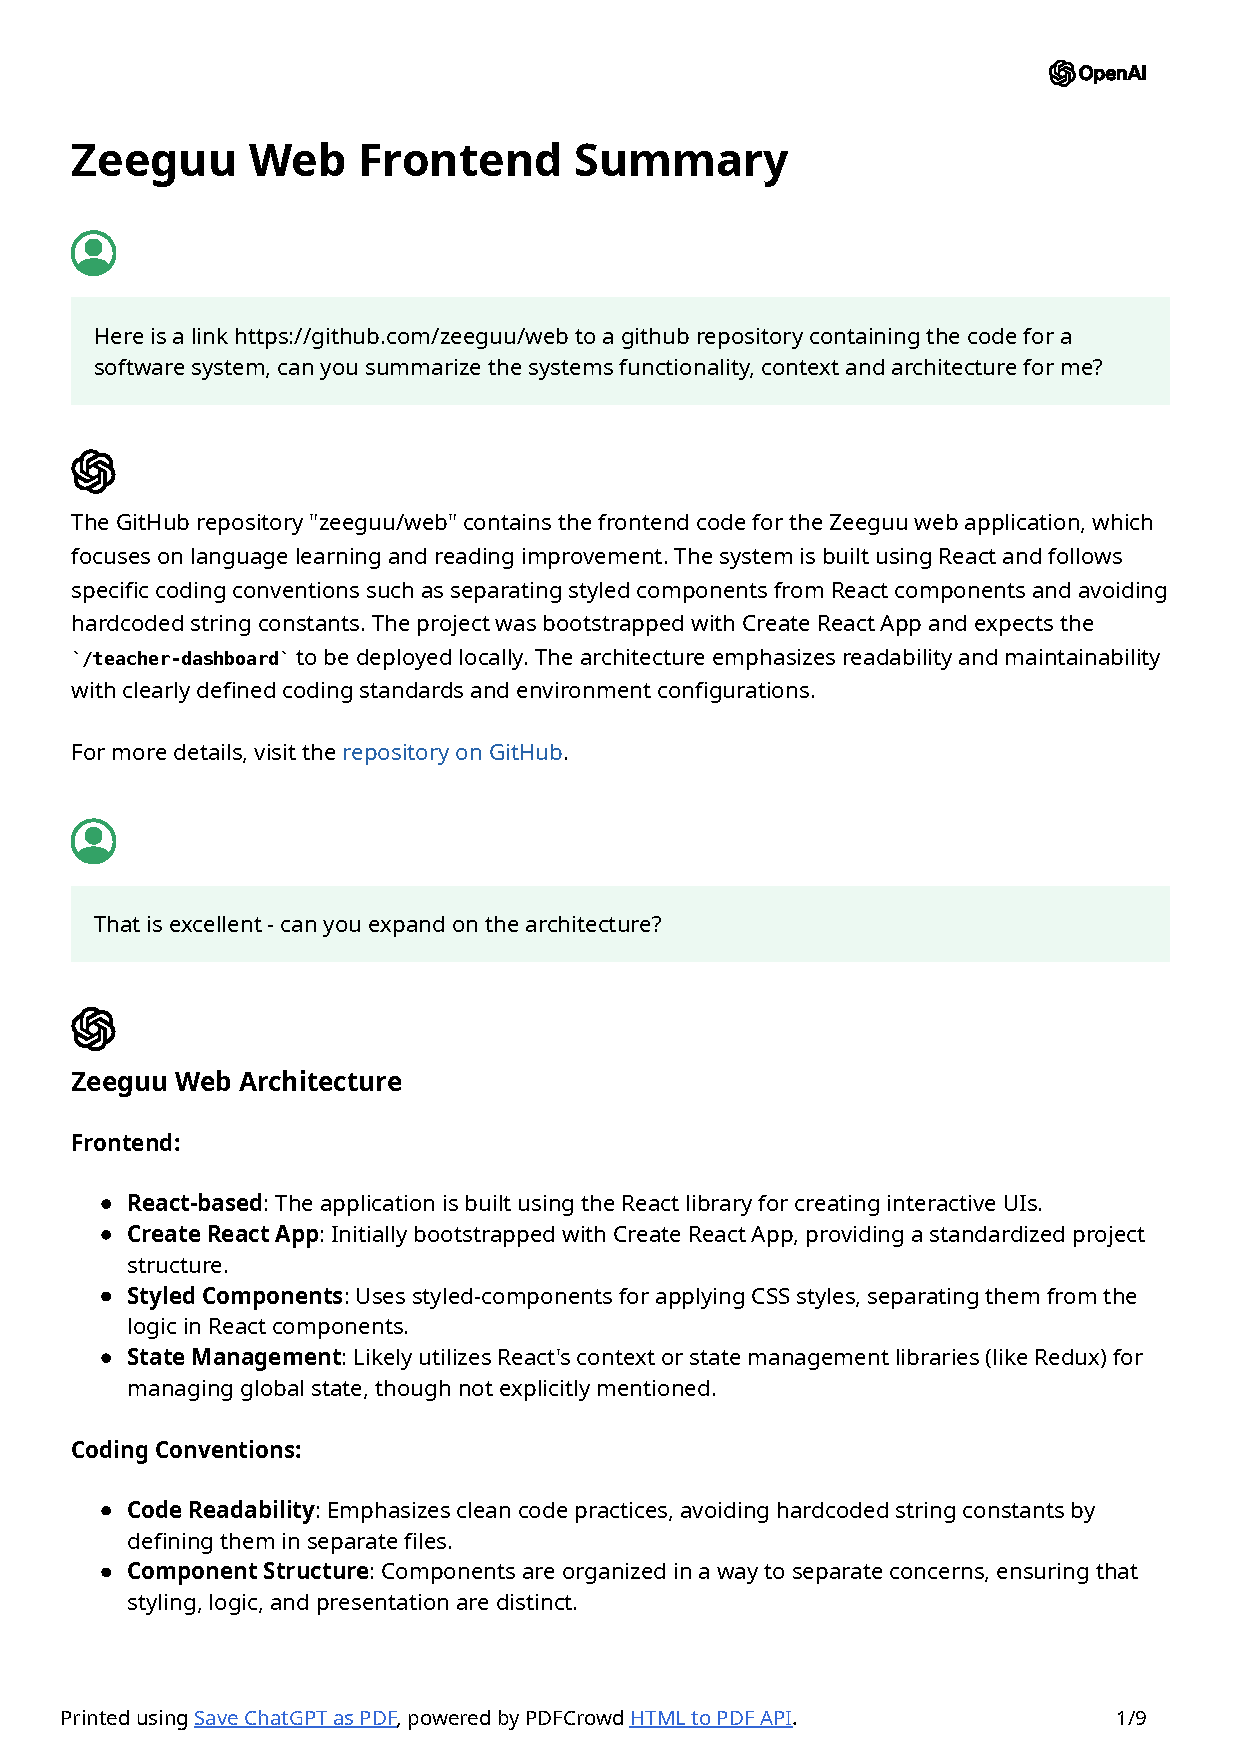
\includepdf[width=\textwidth,pages=1]{appendix/chatgpt.pdf}
\end{figure}
\includepdf[width=\textwidth,pages=2-]{appendix/chatgpt.pdf}

\clearpage
\section{Uploaded Files}
\label{apx:b}
\begin{itemize}
  \item \verb|recovery.zip| -- repository containing code for architectural recovery
\end{itemize}

\clearpage
\section{Approximate Time Allocation}
\label{apx:c}
\begin{itemize}
  \item Development \& tool learning: 60\%
  \item Researching react: 5\%
  \item Playing with/wrangling data: 10\%
  \item Reflecting on results: 10\%
  \item Writing: 15\%
\end{itemize}

\clearpage
\section{Data Visualisation}
\label{apx:d}

\begin{figure}[h]
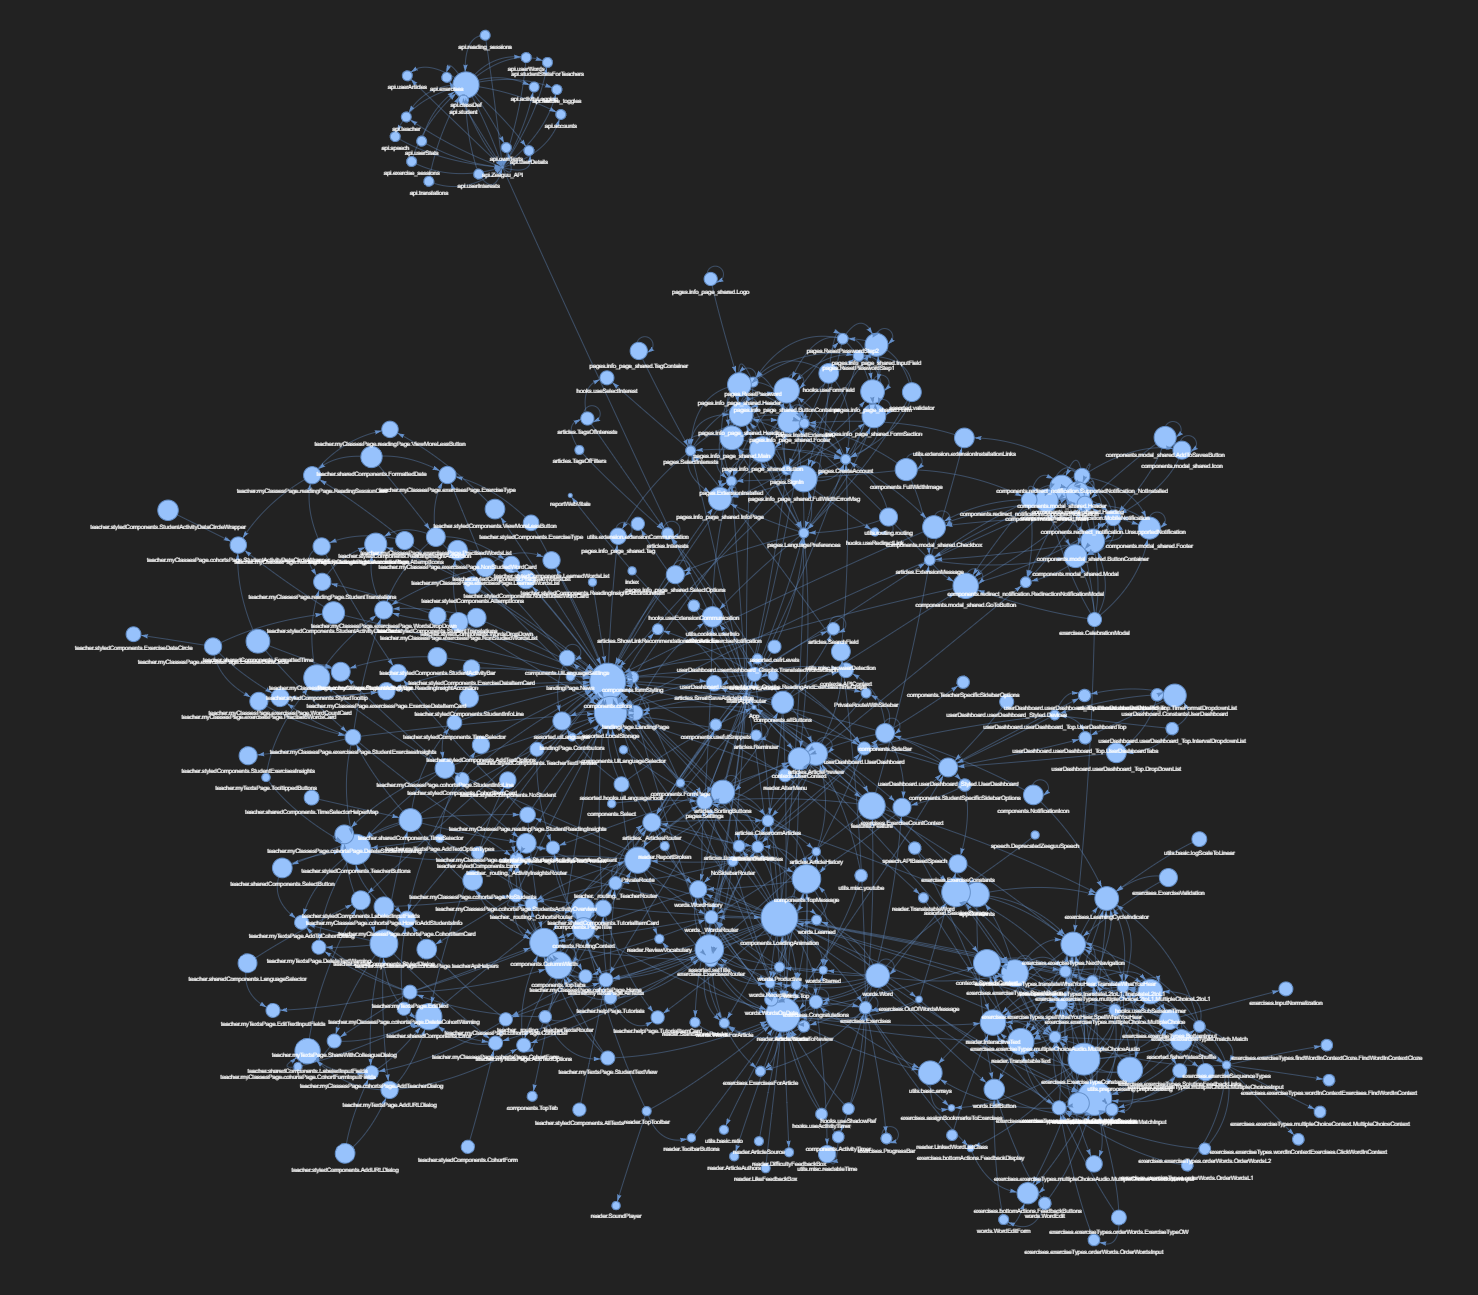
\includegraphics[width=\textwidth]{graphics/raw_imports.png}
\caption{Unfiltered visualisation of all import statements in the sourcecode}
\label{fig:d:raw}
\end{figure}

\begin{figure}[h]
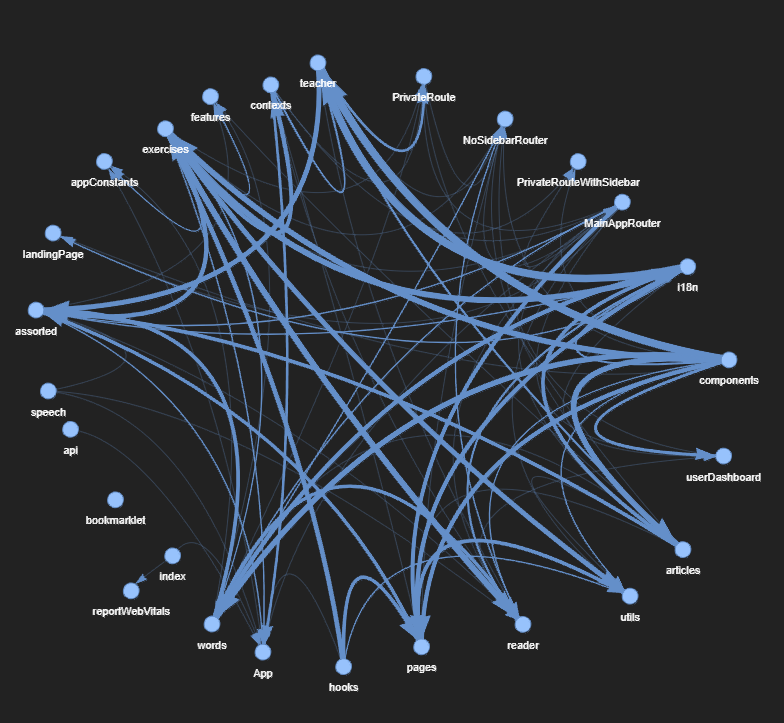
\includegraphics[width=\textwidth]{graphics/module_abstraction_dirty.png}
\caption{Visualisation of all import statements abstracted to top-level modules. 
Thicker edges represent more imports (logarithmically scaled) and edge 
direction represents which what is being imported to where.}
\label{fig:d:abs}
\end{figure}


\begin{figure}[h]
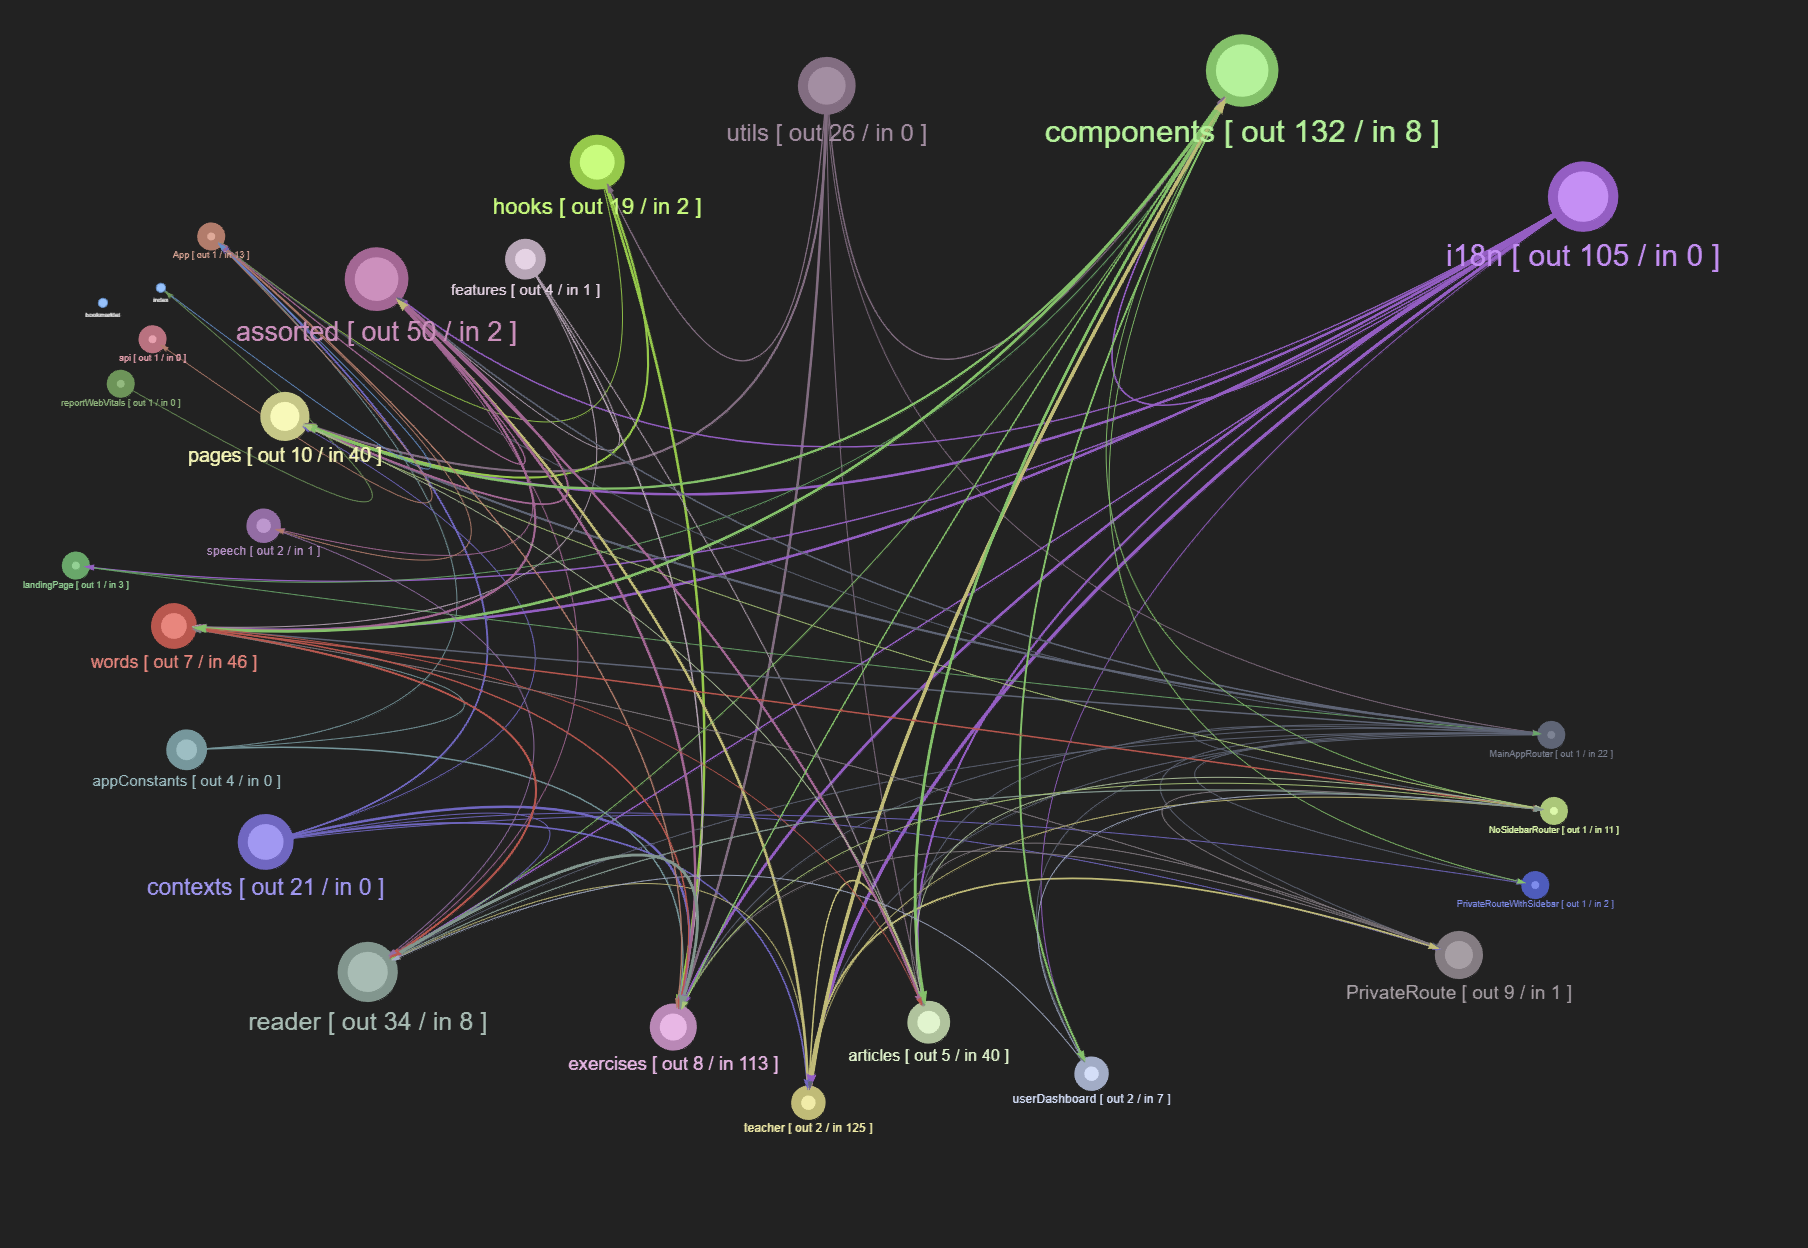
\includegraphics[width=\textwidth]{graphics/module_abstraction_cleaned.png}
\caption{Cleaned and colored visualisation of all import statements abstracted to top-level modules. 
Thicker edges represent more imports (logarithmically scaled) and edge 
direction represents which what is being imported to where.
modules are appended with information about how many times they are imported and how many times they import another module: \\
\hspace*{2em}\textit{out} -- times imported in a different top-level module \\
\hspace*{2em}\textit{in} -- times importing a from different top-level module}
\label{fig:d:clean}
\end{figure}

\begin{figure}[h]
\centering
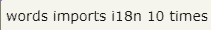
\includegraphics[]{graphics/edge_tooltip.png}
\caption{Tooltip displayed on edges when visualisation is inspected dynamically as .html\\
\hspace*{2em}\textit{out} -- times imported in a different top-level module \\
\hspace*{2em}\textit{in} -- times importing a from different top-level module}
\label{fig:d:edgetooltip}
\end{figure}

\begin{figure}[h]
\centering
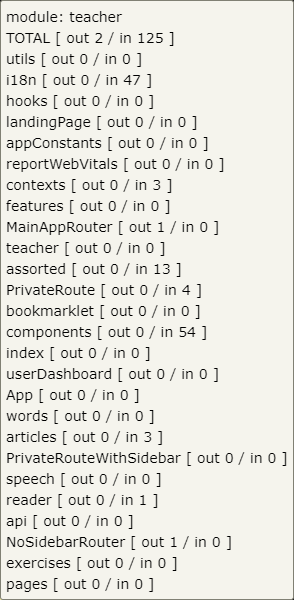
\includegraphics[]{graphics/node_tooltip.png}
\caption{Tooltip displayed on nodes when visualisation is inspected dynamically as .html\\
\hspace*{2em}\textit{out} -- times imported in a different top-level module \\
\hspace*{2em}\textit{in} -- times importing a from different top-level module}
\label{fig:d:nodetooltip}
\end{figure}





\end{document}